\section{Empirical Investigation of \pace}
\label{sec:experiments}


\begin{figure}[t]
    \centering
    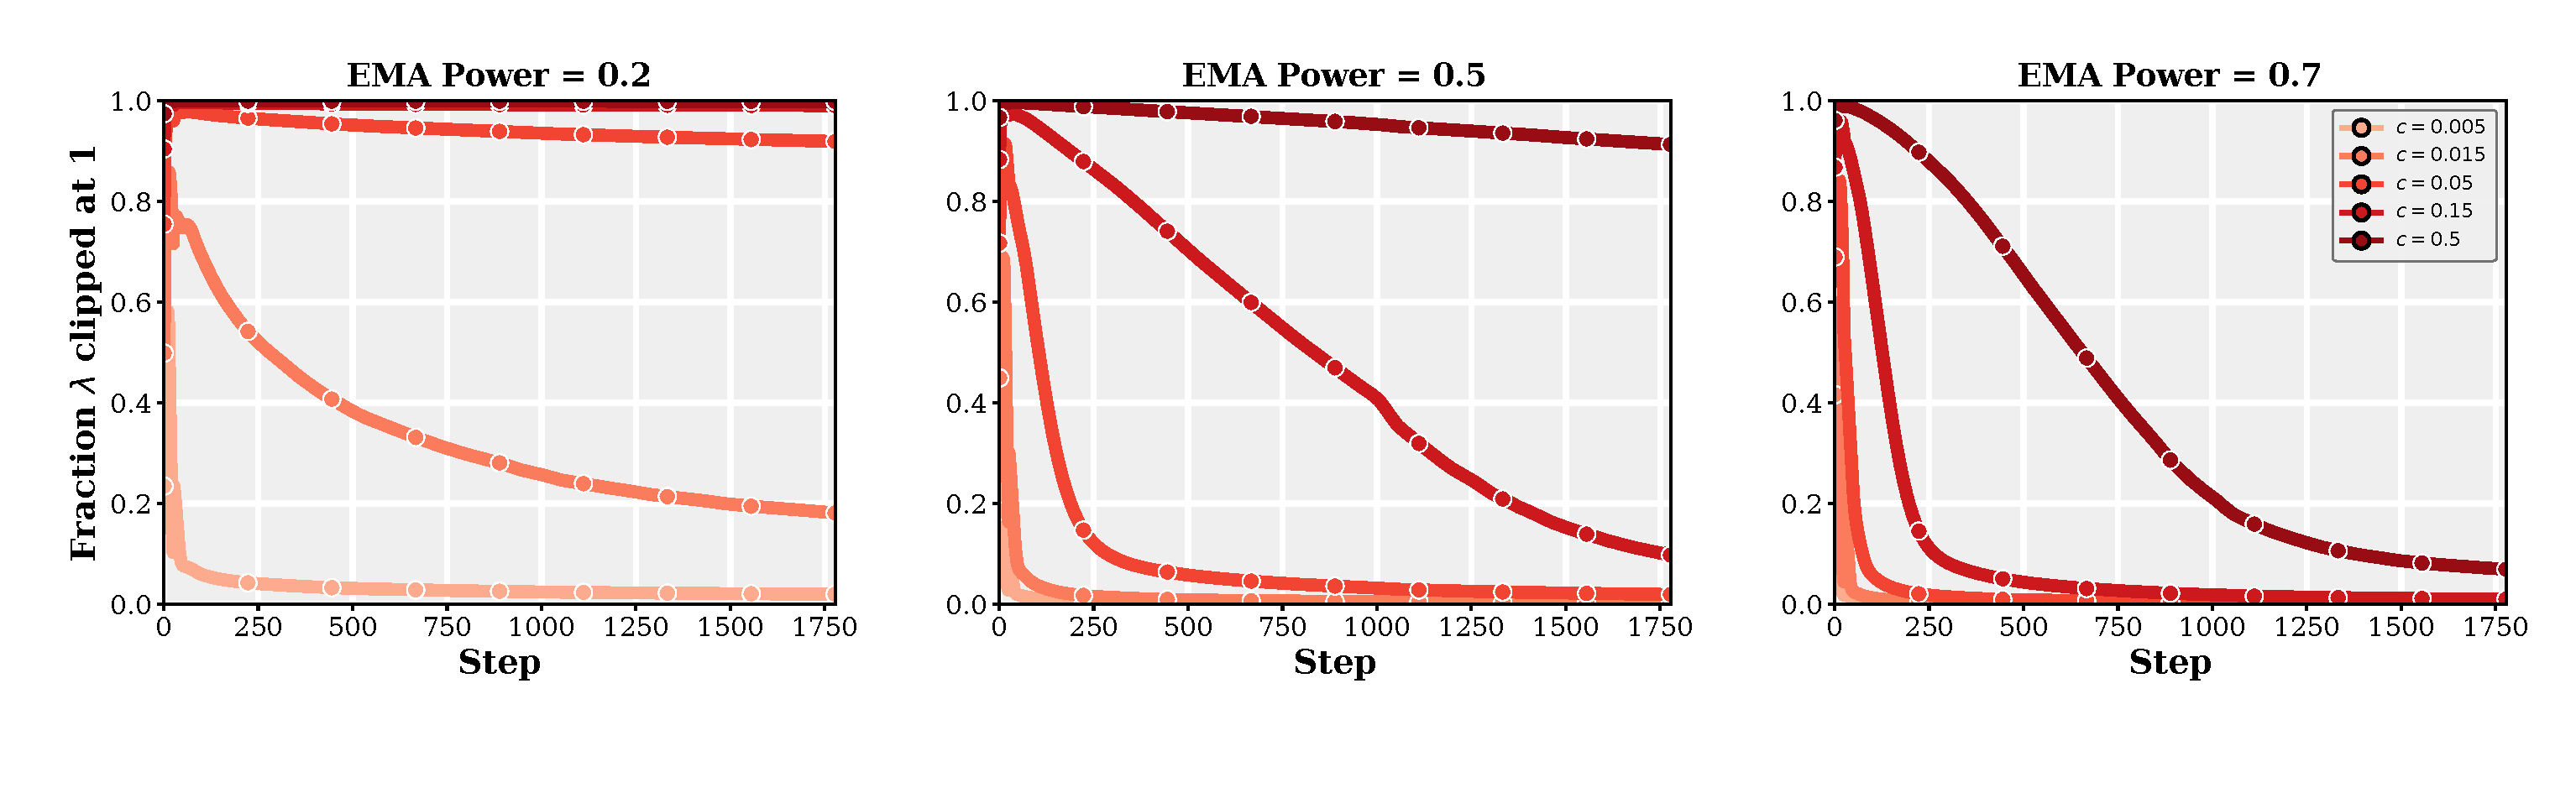
\includegraphics[width=\textwidth]{figures/fig_clip_frac_body.pdf}
    \caption{
        \textbf{Fraction of clipped updates} throughout fine-tuning of SmolLM2-1.7B at a fixed learning rate of $\eta=3{\times}10^{-4}$ for different pullback strengths $c$ and EMA powers $\kappa$.  For large $c$ and small $\kappa$, a substantial fraction of coordinates are clipped at $1$ throughout training, meaning that the pullback fully transports those coordinates to the EMA point, especially early in training.
        }
    \label{fig:clip_frac_body}
\end{figure}


Our proposed algorithm, \pace, was derived in a simplified quadratic model and it is thus not \emph{a priori} clear that it will be effective in practice on the non-convex, non-quadratic problems that arise in language model training.  In this section, we empirically evaluate \pace\ on two standard language-modeling regimes: supervised fine-tuning of openweight $1$--$2$B-parameter language models, and from-scratch pretraining of a $124$M-parameter model at the Chinchilla-optimal token budget. 


Our experiments are primarily organized around three questions: (i) does \pace\ improve on vanilla AdamW and an EMA thereof across model families and learning rates? (ii) is the improvement robust to the optimizer's three new hyperparameters (pullback strength $c$, EMA power $\kappa$, and update frequency $\mathrm{uf}$)? and (iii) how does \pace\ compare to alternative baselines like learning rate decay and Schedule-Free \citep{defazio2024schedule}? Further ablations are deferred to \cref{sec:exp-details}.



\subsection{Empirical Setup}
\label{sec:exp-setup}

For \emph{post-training}, we finetune three pre-trained language models of similar scale, \textbf{SmolLM2-1.7B} \citep{smollm2}, \textbf{Qwen3-1.7B} \citep{qwen3}, and \textbf{Gemma3-1B} \citep{gemma3}, on the \texttt{smol-smoltalk} dataset \citep{smoltalk} for one epoch on the training split, plus a small-model dense ablation on \textbf{SmolLM2-135M}. For \emph{pretraining}, we train \textbf{GPT-2 (124M)} \citep{radford2019gpt2} on \texttt{FineWeb} \citep{penedo2024fineweb} at the Chinchilla-optimal token budget of $2.5$B tokens \citep{hoffmann2022chinchilla}. Fine-tuning runs use a single NVIDIA RTX PRO 6000 GPU; the GPT-2 pretraining sweep runs on a Google Cloud TPU v6e (Trillium) pod, with training hyperparameters and resource costs summarized in and around \cref{tab:models} of \cref{sec:exp-details}. We report final validation cross-entropy on a held-out \texttt{smol-smoltalk} split for fine-tuning and on a fixed FineWeb evaluation shard for pretraining.

\subsection{Main Results}
\label{sec:exp-main}

In \Cref{fig:train_curves}, we show the training curves of \pace, \ema, and vanilla AdamW on the fine-tuning task outlined above.  We see that \pace\ substantially improves on \ema\ at the same per-model learning rate.  Note that the comparison to AdamW without EMA is also included as an illustration.
 In \Cref{fig:pretrain}, we show the \iftoggle{colt}{}{same comparison for the} pretraining regime, where we again see a clear improvement of \pace\ over \ema.  
 In \Cref{fig:appendix_tulu_qwen} (deferred to the appendix), we repeat these experiments for Qwen on the Tulu dataset \citep{lambert2024tulu}, with similar results.
In all cases, we compare the best configurations of \ema\ and vanilla training to \pace, where we swept across learning rate, decay schedule, EMA power $\kappa$, and pullback strength $c$ to find the best configuration for each baseline.  Thus, these results suggest that \pace\ can significantly improve on the performance of the iterate-average estimator in practice, and that this improvement is robust across model families and datasets.





\subsection{Further Empirical Results}
\label{sec:exp-further}

In addition to our main results, we also conduct a number of ablations and further experiments to better understand the behavior of \pace\ and its sensitivity to its hyperparameters.  While many results are deferred to \cref{sec:exp-details} in the interest of space, we briefly summarize some of the key findings.

\paragraph{Effect of pullback strength $c$, EMA power $\kappa$, and update frequency.}  In each of our settings, we conduct a dense sweep over the pullback strength $c$ and EMA power $\kappa$ hyperparameters of \pace\ for several learning rates and update frequencies in order to understand the sensitivity of \pace\ to these hyperparameters and to verify that the improvement over EMA-evaluated AdamW is robust.  An example from our fine-tuning experiments is shown in \Cref{fig:135m_grid}, which is broadly replicated across models and settings (\Cref{fig:c_kappa,fig:appendix_135m_full_grid}).  In particular, we see that relatively small values of $c$ (e.g. $c=3 \times 10^{-3}$) can substantially improve on EMA-evaluated AdamW, and that the improvement is robust across a range of learning rates and update frequencies.




\paragraph{Effect of clipping $\lambda$.}  In \eqref{eq:practical_control_strategy_empirical} and \Cref{alg:controlled-bema}, we clip the pullback gain $\lambda$ to ensure that the update is always a convex combination of the iterate average and the na{\"i}ve optimizer step.  When the clipping is instantiated, \pace\ transports the relevant coordinate of the current iterate $\theta_k$ to exactly equal that of the EMA point $\thetema[k]$, recovering a special case of Lookahead \citep{zhang2019lookahead}.  In \cref{fig:clip_frac_body}, we show how the fraction of clipped coordinates varies with different hyperparameters throughout training on SmolLM2-1.7B at $\eta=3{\times}10^{-4}$, observing that in extreme cases, essentially all coordinates are clipped (especially early in training), but generally clipping is not enforced for most coordinates.  \iftoggle{colt}{}{
Further results are in \cref{fig:appendix_clip_frac,fig:appendix_clip_frac_vs_c}.
}

\paragraph{Effect of LR Decay.} 
While our theory assumed constant learning rate, decay schedules are a standard part of practical training pipelines.  We experiment with three decay schedules: (i) constant learning rate, (ii) linear decay to zero over the last $20\%$ of steps, and (iii) cosine decay to zero.  In  \Cref{fig:pretrain} (right) we compare \pace\ to AdamW with linear decay to zero over the last $20\%$ of steps in pretraining, finding that \pace\ strictly improves even in this setting.  Exhaustive results for all three schedules can be found in \Cref{sec:exp-details,sec:app-post}; in summary, \pace\ provides improvement over the baseline across all schedules, and the improvement is robust to the choice of schedule.










\paragraph{Comparing to the schedule-free baseline.} We also compare \pace\ to the most prominent schedule-free optimizer (SF) \citep{defazio2024schedule}, which also uses iterate averaging to stabilize training and remove the need for learning rate decay.  In \Cref{fig:bema_sf}, we compare \pace\ to Schedule-Free and observe competitive performance. While Schedule-Free requires one fewer copy of model weights than our na{\"i}ve \pace\ implementation, it must switch between `fast' and `slow' moving iterate averages during training, leading to slower training (12 vs 10 hours on a v6e TPU for Qwen3-1.7B in our experiments).  Finally, in \Cref{fig:bema_sf} (right), we show that \pace\ applied with a constant learning rate outperforms AdamW with WSD at every token budget, suggesting that \pace\ can be an effective alternative to learning rate decay.  Similar results hold for pretraining, as shown in \Cref{fig:appendix_pretrain_river}, providing further evidence that \pace\ can be an effective alternative to learning rate decay, although we emphasize that improved performance is typically achieved by combining \pace\ with a decay schedule.






\begin{figure}[t]
    \centering
    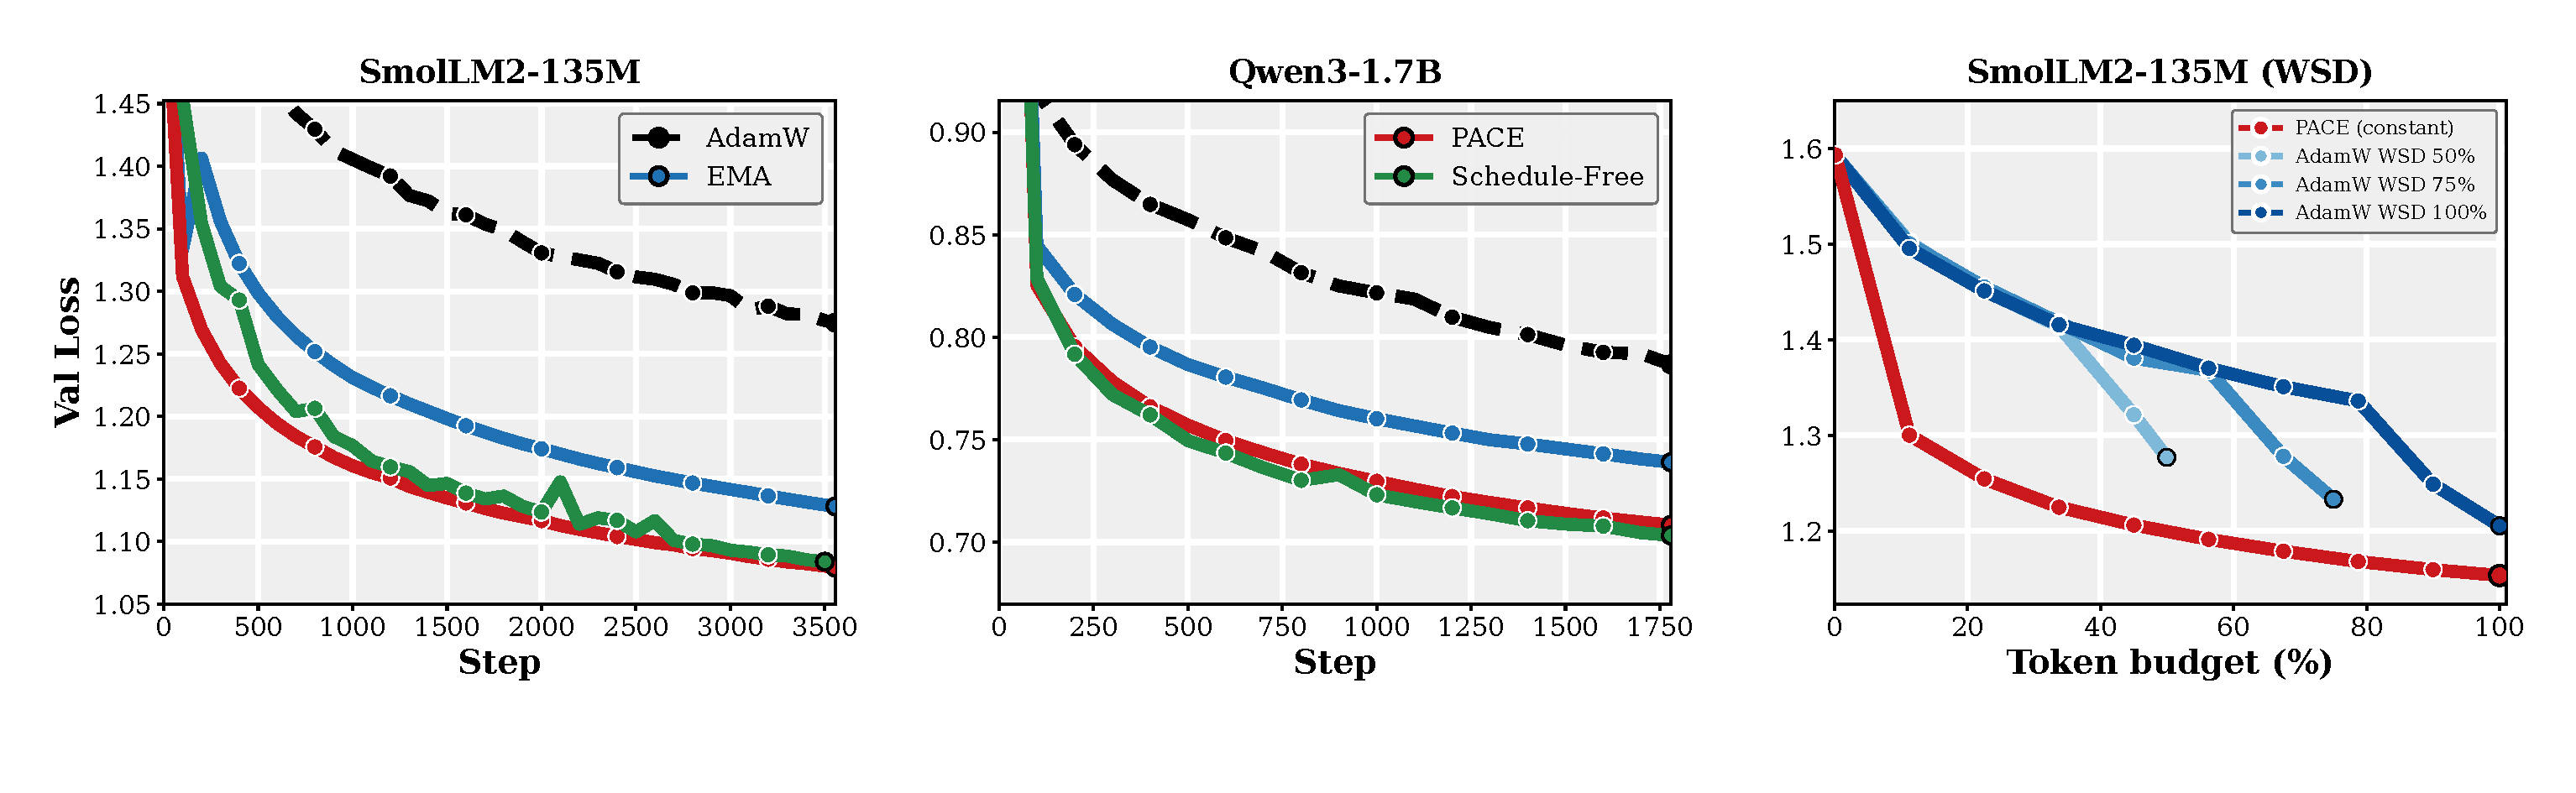
\includegraphics[width=\textwidth]{figures/fig4_bema_sf.pdf}
    \caption{
        \textbf{Comparison of \pace\ to Schedule-Free \citep{defazio2024schedule}, AdamW, and EMA on fine-tuning.} Validation cross-entropy on \texttt{smol-smoltalk} for SmolLM2-135M (\textbf{left}), Qwen3-1.7B (\textbf{middle}), and a token-budget comparison on SmolLM2-135M (\textbf{right}): AdamW with WSD decays the learning rate to zero over the last $20\%$ of token budgets of $50\%/75\%/100\%$ of the run, while \pace\ trains at a constant learning rate over the full budget. \pace\ improves on AdamW and EMA-only and is competitive with Schedule-Free; in the right panel, every WSD branch ends above the \pace\ trajectory at every budget.
        }
    \label{fig:bema_sf}
\end{figure}
